\documentclass{standalone}
\usepackage{tikz}
\usetikzlibrary{patterns, positioning}


\begin{document}
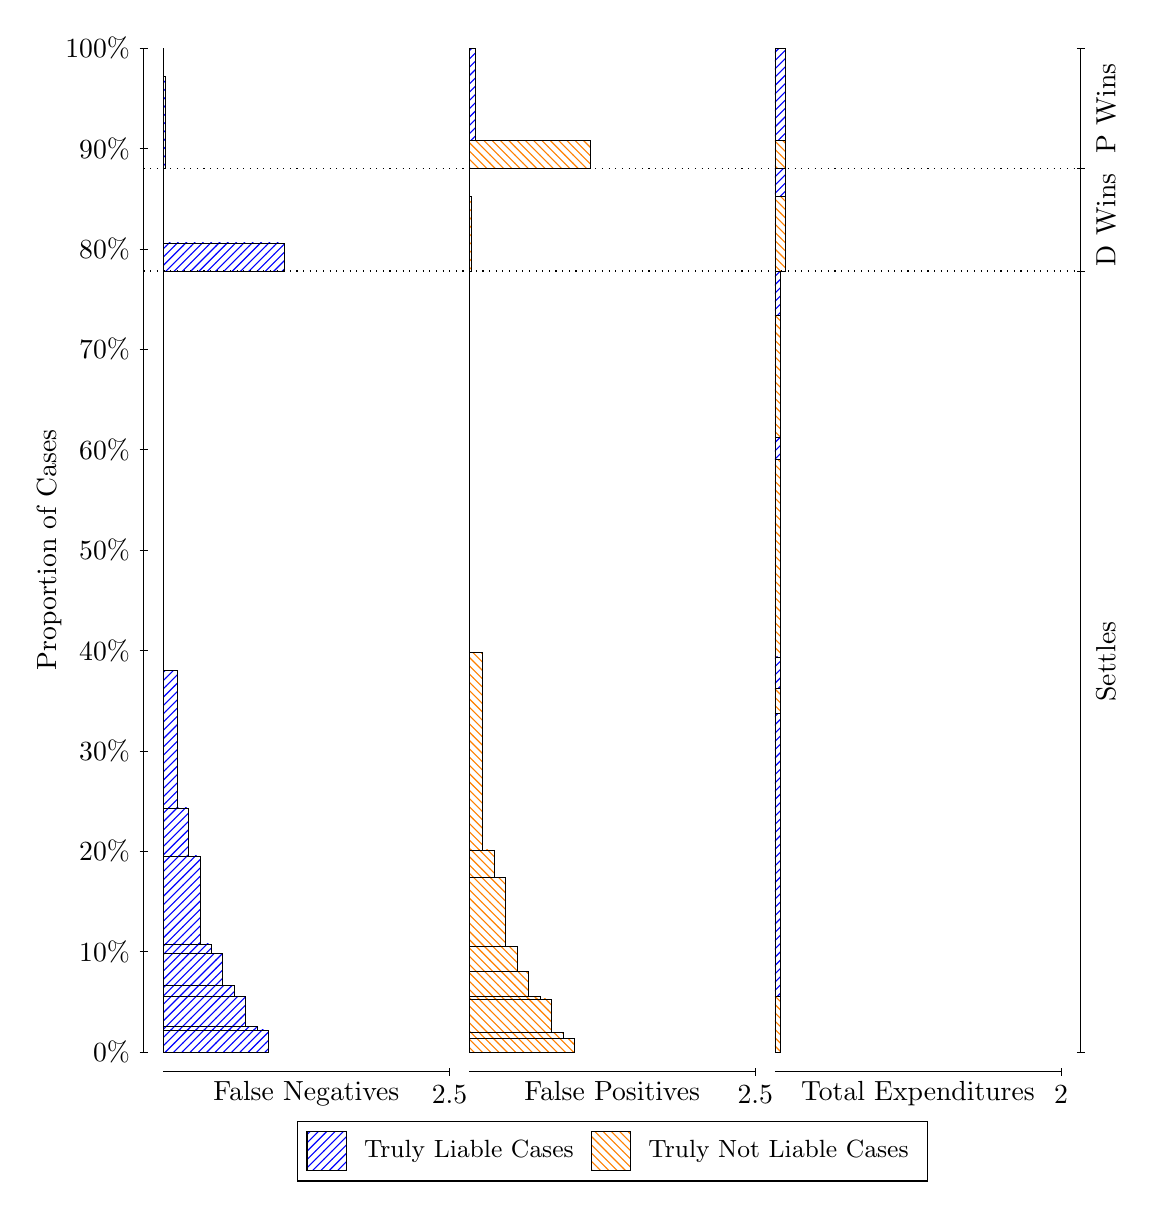
\begin{tikzpicture}
\draw[black, very thin] (1.5,1.75) -- (1.5,14.5);
\node[rotate=90, text=black, anchor=center] at (0.3, 8.125) {Proportion of Cases};
\draw[black, very thin] (1.45,1.75) -- (1.55,1.75);
\node[text=black, anchor=east] at (1.45, 1.75) {0\%};
\draw[black, very thin] (1.45,3.025) -- (1.55,3.025);
\node[text=black, anchor=east] at (1.45, 3.025) {10\%};
\draw[black, very thin] (1.45,4.3) -- (1.55,4.3);
\node[text=black, anchor=east] at (1.45, 4.3) {20\%};
\draw[black, very thin] (1.45,5.575) -- (1.55,5.575);
\node[text=black, anchor=east] at (1.45, 5.575) {30\%};
\draw[black, very thin] (1.45,6.85) -- (1.55,6.85);
\node[text=black, anchor=east] at (1.45, 6.85) {40\%};
\draw[black, very thin] (1.45,8.125) -- (1.55,8.125);
\node[text=black, anchor=east] at (1.45, 8.125) {50\%};
\draw[black, very thin] (1.45,9.4) -- (1.55,9.4);
\node[text=black, anchor=east] at (1.45, 9.4) {60\%};
\draw[black, very thin] (1.45,10.675) -- (1.55,10.675);
\node[text=black, anchor=east] at (1.45, 10.675) {70\%};
\draw[black, very thin] (1.45,11.95) -- (1.55,11.95);
\node[text=black, anchor=east] at (1.45, 11.95) {80\%};
\draw[black, very thin] (1.45,13.225) -- (1.55,13.225);
\node[text=black, anchor=east] at (1.45, 13.225) {90\%};
\draw[black, very thin] (1.45,14.5) -- (1.55,14.5);
\node[text=black, anchor=east] at (1.45, 14.5) {100\%};

\draw[black, very thin] (13.4,1.75) -- (13.4,14.5);
\draw[black, very thin] (13.35,1.75) -- (13.45,1.75);
\node[anchor=west] at (13.35, 1.75) {};
\draw[black, very thin] (13.35,11.668) -- (13.45,11.668);
\node[anchor=west] at (13.35, 11.668) {};
\draw[black, very thin] (13.35,12.969) -- (13.45,12.969);
\node[anchor=west] at (13.35, 12.969) {};
\draw[black, very thin] (13.35,14.5) -- (13.45,14.5);
\node[anchor=west] at (13.35, 14.5) {};

\draw[black, very thin, pattern color=blue, pattern=north east lines] (1.75,1.75) rectangle (3.0852,2.0315);
\draw[black, very thin, pattern color=blue, pattern=north east lines] (1.75,2.0315) rectangle (2.9399,2.0798);
\draw[black, very thin, pattern color=blue, pattern=north east lines] (1.75,2.0798) rectangle (2.7946,2.4521);
\draw[black, very thin, pattern color=blue, pattern=north east lines] (1.75,2.4521) rectangle (2.6492,2.5994);
\draw[black, very thin, pattern color=blue, pattern=north east lines] (1.75,2.5994) rectangle (2.5039,3.0029);
\draw[black, very thin, pattern color=blue, pattern=north east lines] (1.75,3.0029) rectangle (2.3586,3.1228);
\draw[black, very thin, pattern color=blue, pattern=north east lines] (1.75,3.1228) rectangle (2.2133,4.2392);
\draw[black, very thin, pattern color=blue, pattern=north east lines] (1.75,4.2392) rectangle (2.0679,4.8486);
\draw[black, very thin, pattern color=blue, pattern=north east lines] (1.75,4.8486) rectangle (1.9226,6.5952);
\draw[black, very thin, pattern color=orange, pattern=north west lines] (1.75,6.5952) rectangle (1.75,11.668);
\draw[black, very thin, pattern color=blue, pattern=north east lines] (1.75,11.668) rectangle (3.2851,12.026);
\draw[black, very thin, pattern color=orange, pattern=north west lines] (1.75,12.026) rectangle (1.75,12.969);
\draw[black, very thin, pattern color=blue, pattern=north east lines] (1.75,12.969) rectangle (1.7773,14.141);
\draw[black, very thin, pattern color=orange, pattern=north west lines] (1.75,14.141) rectangle (1.75,14.5);
\draw[black, very thin, pattern color=orange, pattern=north west lines] (5.6333,1.75) rectangle (6.9686,1.9243);
\draw[black, very thin, pattern color=orange, pattern=north west lines] (5.6333,1.9243) rectangle (6.8233,2.0002);
\draw[black, very thin, pattern color=orange, pattern=north west lines] (5.6333,2.0002) rectangle (6.6779,2.4244);
\draw[black, very thin, pattern color=orange, pattern=north west lines] (5.6333,2.4244) rectangle (6.5326,2.4548);
\draw[black, very thin, pattern color=orange, pattern=north west lines] (5.6333,2.4548) rectangle (6.3873,2.7723);
\draw[black, very thin, pattern color=orange, pattern=north west lines] (5.6333,2.7723) rectangle (6.2419,3.0952);
\draw[black, very thin, pattern color=orange, pattern=north west lines] (5.6333,3.0952) rectangle (6.0966,3.9639);
\draw[black, very thin, pattern color=orange, pattern=north west lines] (5.6333,3.9639) rectangle (5.9513,4.3178);
\draw[black, very thin, pattern color=orange, pattern=north west lines] (5.6333,4.3178) rectangle (5.8059,6.8231);
\draw[black, very thin, pattern color=blue, pattern=north east lines] (5.6333,6.8231) rectangle (5.6333,11.668);
\draw[black, very thin, pattern color=orange, pattern=north west lines] (5.6333,11.668) rectangle (5.6606,12.611);
\draw[black, very thin, pattern color=blue, pattern=north east lines] (5.6333,12.611) rectangle (5.6333,12.969);
\draw[black, very thin, pattern color=orange, pattern=north west lines] (5.6333,12.969) rectangle (7.1684,13.328);
\draw[black, very thin, pattern color=blue, pattern=north east lines] (5.6333,13.328) rectangle (5.7151,14.5);
\draw[black, very thin, pattern color=orange, pattern=north west lines] (9.5167,1.75) rectangle (9.5848,2.4548);
\draw[black, very thin, pattern color=blue, pattern=north east lines] (9.5167,2.4548) rectangle (9.5848,6.047);
\draw[black, very thin, pattern color=orange, pattern=north west lines] (9.5167,6.047) rectangle (9.5848,6.3646);
\draw[black, very thin, pattern color=blue, pattern=north east lines] (9.5167,6.3646) rectangle (9.5848,6.7681);
\draw[black, very thin, pattern color=orange, pattern=north west lines] (9.5167,6.7681) rectangle (9.5848,9.2733);
\draw[black, very thin, pattern color=blue, pattern=north east lines] (9.5167,9.2733) rectangle (9.5848,9.5548);
\draw[black, very thin, pattern color=orange, pattern=north west lines] (9.5167,9.5548) rectangle (9.5848,11.1);
\draw[black, very thin, pattern color=blue, pattern=north east lines] (9.5167,11.1) rectangle (9.5848,11.668);
\draw[black, very thin, pattern color=orange, pattern=north west lines] (9.5167,11.668) rectangle (9.6529,12.611);
\draw[black, very thin, pattern color=blue, pattern=north east lines] (9.5167,12.611) rectangle (9.6529,12.969);
\draw[black, very thin, pattern color=orange, pattern=north west lines] (9.5167,12.969) rectangle (9.6529,13.328);
\draw[black, very thin, pattern color=blue, pattern=north east lines] (9.5167,13.328) rectangle (9.6529,14.5);
\draw[black, dotted] (1.5,11.668) -- (13.4,11.668);
\draw[black, dotted] (1.5,12.969) -- (13.4,12.969);
\draw[black, very thin] (1.75,1.5) -- (5.3833,1.5);
\node[text=black, anchor=north] at (3.5667, 1.5) {False Negatives};
\draw[black, very thin] (5.3833,1.45) -- (5.3833,1.55);
\node[text=black, anchor=north] at (5.3833, 1.45) {2.5};

\draw[black, very thin] (5.6333,1.5) -- (9.2667,1.5);
\node[text=black, anchor=north] at (7.45, 1.5) {False Positives};
\draw[black, very thin] (9.2667,1.45) -- (9.2667,1.55);
\node[text=black, anchor=north] at (9.2667, 1.45) {2.5};

\draw[black, very thin] (9.5167,1.5) -- (13.15,1.5);
\node[text=black, anchor=north] at (11.333, 1.5) {Total Expenditures};
\draw[black, very thin] (13.15,1.45) -- (13.15,1.55);
\node[text=black, anchor=north] at (13.15, 1.45) {2};

\node[text=black, centered, rotate=90] at (13.72, 6.7091) {Settles};
\node[text=black, centered, rotate=90] at (13.72, 12.319) {D Wins};
\node[text=black, centered, rotate=90] at (13.72, 13.734) {P Wins};

\draw (7.449999999999999,1.5) node[draw=none] (baseCoordinate) {};
\begin{scope}[align=center]
        \matrix[scale=0.5, draw=black, below=0.5cm of baseCoordinate, nodes={draw}, column sep=0.1cm]{
            \node[rectangle, draw, minimum width=0.5cm, minimum height=0.5cm, pattern color=blue, pattern=north east lines] {}; &
            \node[draw=none, font=\small, text=black] (B) {Truly Liable Cases}; &
            \node[rectangle, draw, minimum width=0.5cm, minimum height=0.5cm, pattern color=orange, pattern=north west lines] {}; &
            \node[draw=none, font=\small, text=black] (B) {Truly Not Liable Cases}; \\
            };
\end{scope}

\end{tikzpicture}
\end{document}